
The multidimensional mapping algorithm aims at translating a multidimensional geometry into an imaginary 1D strand. This procedure serves allows for $(i)$ assigning the~magnetic field to the~windings separately, $(ii)$ mapping the~geometry for the~quench detection algorithm. 

As illustrated in Fig.~\ref{fig: 3d_coil_illustation_with_2d_b_field}, a multi-strand domain is subjected to a time- and space-dependent magnetic field. Thus, every winding is exposed to a different magnetic field which also varies with a current change. From the magnetic analysis standpoint, it is assumed that the coil is infinitely long, allowing for using a 2D magnetic map from the centre of a~magnet cross-section.

\begin{figure}[H]
    \centering
    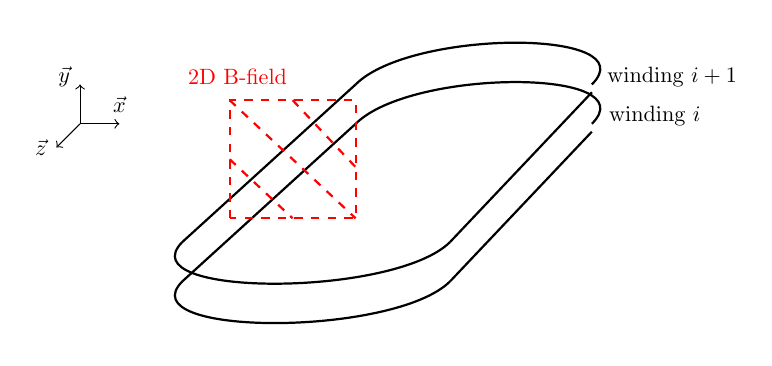
\begin{tikzpicture}[scale = 1]
        
        \foreach \y in {0,0.5} 
        \draw[thick,  black] (0.2,\y) -- (2,\y+1.9);
        \foreach \y in {0,0.5} 
        \draw[thick, black] (.2,\y) .. controls +(45:-1cm) and +(45:-1cm) .. (-3.2,\y);
        \foreach \y in {0,0.5} 
        \draw[thick,  black] (-3.2,\y) -- (-1,\y+2.0);
        \foreach \y in {0,0.5} 
        \draw[thick, black] (-1,\y+2) .. controls +(45:1cm) and +(45:1cm) .. (2,\y+2);
        
        \draw[thick, dashed, red] (-2.6,0.8) rectangle (-1.0,2.3);
        \draw[thick, dashed, red] (-2.6,1.55) -- (-1.8, 0.8);
        \draw[thick, dashed, red] (-2.6,2.3) -- (-1.0, 0.8);
        \draw[thick, dashed, red] (-1.8,2.3) -- (-1.0, 1.45);
        
        \node[scale = 0.8] at (2.8,2.1) {winding $i$};
        \node[scale = 0.8] at (3.02,2.6) {winding $i+1$};
        \node[red, scale = 0.8] at (-2.5,2.6) {2D B-field};
        
        \draw[black, ->] (-4.5,2) -- (-4.8,1.7);
        \draw[black, ->] (-4.5,2) -- (-4.5,2.5);
        \draw[black, ->] (-4.5,2) -- (-4,2);
        
        \node[scale = 0.8] at (-4,2.25) {$\vec{x}$};
        \node[scale = 0.8] at (-4.7,2.6) {$\vec{y}$};
        \node[scale = 0.8] at (-5,1.7) {$\vec{z}$};
        
    \end{tikzpicture}
    \caption{Schematic of an assignment of a magnetic field to a multi-strand domain.}
    \label{fig: 3d_coil_illustation_with_2d_b_field}
\end{figure}

The magnetic field is assigned to every winding separately, as shown in Fig.~\ref{fig:ansys_python_mapping scheme}. Each of them is characterised by a different thermal and electrical material property. The multi-strand geometry is translated into a realistic one-dimensional cable with a length $L_\text{coil}$ equal to the total coil length. Each part of the coil corresponding to one winding, is subjected to a~different magnetic field~$B_\text{n}$. Similarly to Fig.~\ref{fig: 1d_strand_geometry}, the one-dimensional coordinate system $\bar x$ in Fig.~\ref{fig:ansys_python_mapping scheme} represents the~longitudinal direction of the coil. 

\begin{figure}[H]
\centering
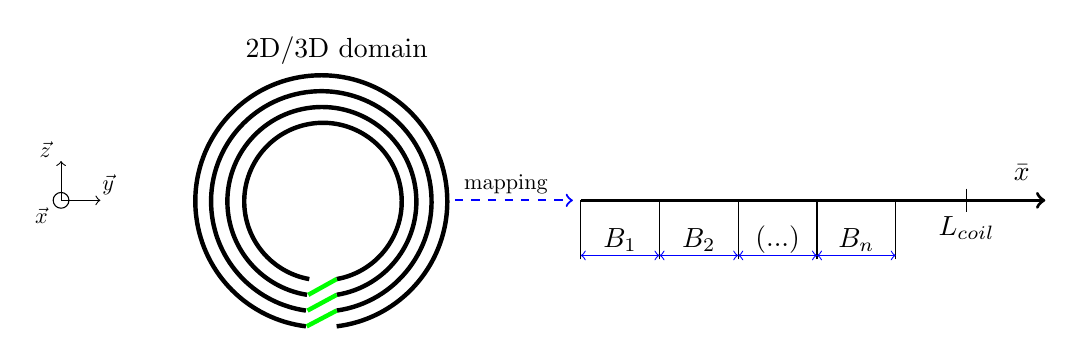
\begin{tikzpicture}[scale = 1]
\draw [ultra thick] (0,0) arc (-80:260:1);
\draw [ultra thick] (0,-0.2) arc (-81:261:1.2);
\draw [ultra thick] (0,-0.4) arc (-82:262:1.4);
\draw [ultra thick] (0,-0.6) arc (-83:263:1.6);
\draw [ultra thick, green] (0,0) -- (-0.36,-0.2);
\draw [ultra thick, green] (0,-0.2) -- (-0.37,-0.4);
\draw [ultra thick, green] (0,-0.4) -- (-0.38,-0.6);
\node[scale = 1.0] at (0,2.9) {2D/3D domain};
\draw [thick, dashed, blue, ->] (1.5,1) -- (3,1);
\node[scale = 0.8] at (2.15,1.2) {mapping};
\draw [very thick, ->] (3.1,1) -- (9,1);
\foreach \t in {3.1, 4.1, ..., 7.1}
\draw [thin] ({\t},0.25) -- ({\t},1);
\foreach \t in {3.1, 4.1, ..., 6.1}
\draw [thin, blue, <->] ({\t},0.3) -- ({\t+1},0.3);

\draw [thin] (8.0,1.15) -- (8.0,0.85);

\node[scale = 1.0] at (3.6,0.5) {$B_1$};
\node[scale = 1.0] at (4.6,0.5) {$B_2$};
\node[scale = 1.0] at (5.6,0.5) {(...)};
\node[scale = 1.0] at (6.6,0.5) {$B_\text{n}$};
\node[scale = 1.0] at (8,0.65) {$L_\text{coil}$};

\node[scale = 1.0] at (8.7,1.35) {$\bar x$};

\draw (-3.5,1) circle (0.1cm);
\draw[black, ->] (-3.5,1) -- (-3.5,1.5);
\draw[black, ->] (-3.5,1) -- (-3,1);

\node[scale = 0.8] at (-3.75,0.8) {$\vec{x}$};
\node[scale = 0.8] at (-2.9,1.2) {$\vec{y}$};
\node[scale = 0.8] at (-3.7,1.65) {$\vec{z}$};

\end{tikzpicture}
\caption{Mapping scheme of a magnetic field onto an imaginary 1D coil.}
\label{fig:ansys_python_mapping scheme}
\end{figure}

